\chapter{Levantamento de Requisitos}

Com a recolha de todos os dados necessários para o desenvolvimento do projeto, é possível identificar as fragilidades de outros \textit{softwares} desenvolvidos presentes no mercado, dando assim uma melhor perceção daquilo que poderá ser melhorado ou até mesmo implementado, sendo uma inovação para o setor. Assim, fazer o levantamento de requisitos e estabelecer o primeiro contacto com o tema em questão, é o primeiro passo a ser desenvolvido.

\section{Técnicas de Levantamento de Requisitos}
De forma a levantar os requisitos eficazmente decidimos fazer um inquérito ao público alvo da nossa aplicação, todos os indivíduos maiores de 18 anos, com questões relevantes acerca do que deverá constar num bom sistema de apostas.
\subsection{Questionário ao público alvo}
\begin{enumerate}
    \item Em que desportos gostavam mais de apostar?
        \begin{enumerate}
            \item Futebol
            \item Andebol
            \item Basquetebol 
            \item Hóquei em Patins
            \item Ténis
            \item MotoGP
            \item Futsal
            \item Futebol Americano
            \item Fórmula 1
            \item Voleibol 
        \end{enumerate}
    \item Gostavam de apostar em...
        \begin{enumerate}
            \item Vitória, derrota e empate
            \item Opções acima e número de golos
            \item Opções acima e que jogador marca cada golo
        \end{enumerate}
    \item Gostavam de ter hipótese de fazer mais de uma aposta simultaneamente?
        \begin{enumerate}
            \item Sim
            \item Não
        \end{enumerate}
     
\end{enumerate}

\newpage
\subsubsection{Respostas Obtidas}
\vspace{5mm}
\begin{enumerate}
    \item \textbf{Em que desportos gostavam mais de apostar?}
        \begin{figure}[!htb]
            \centering
            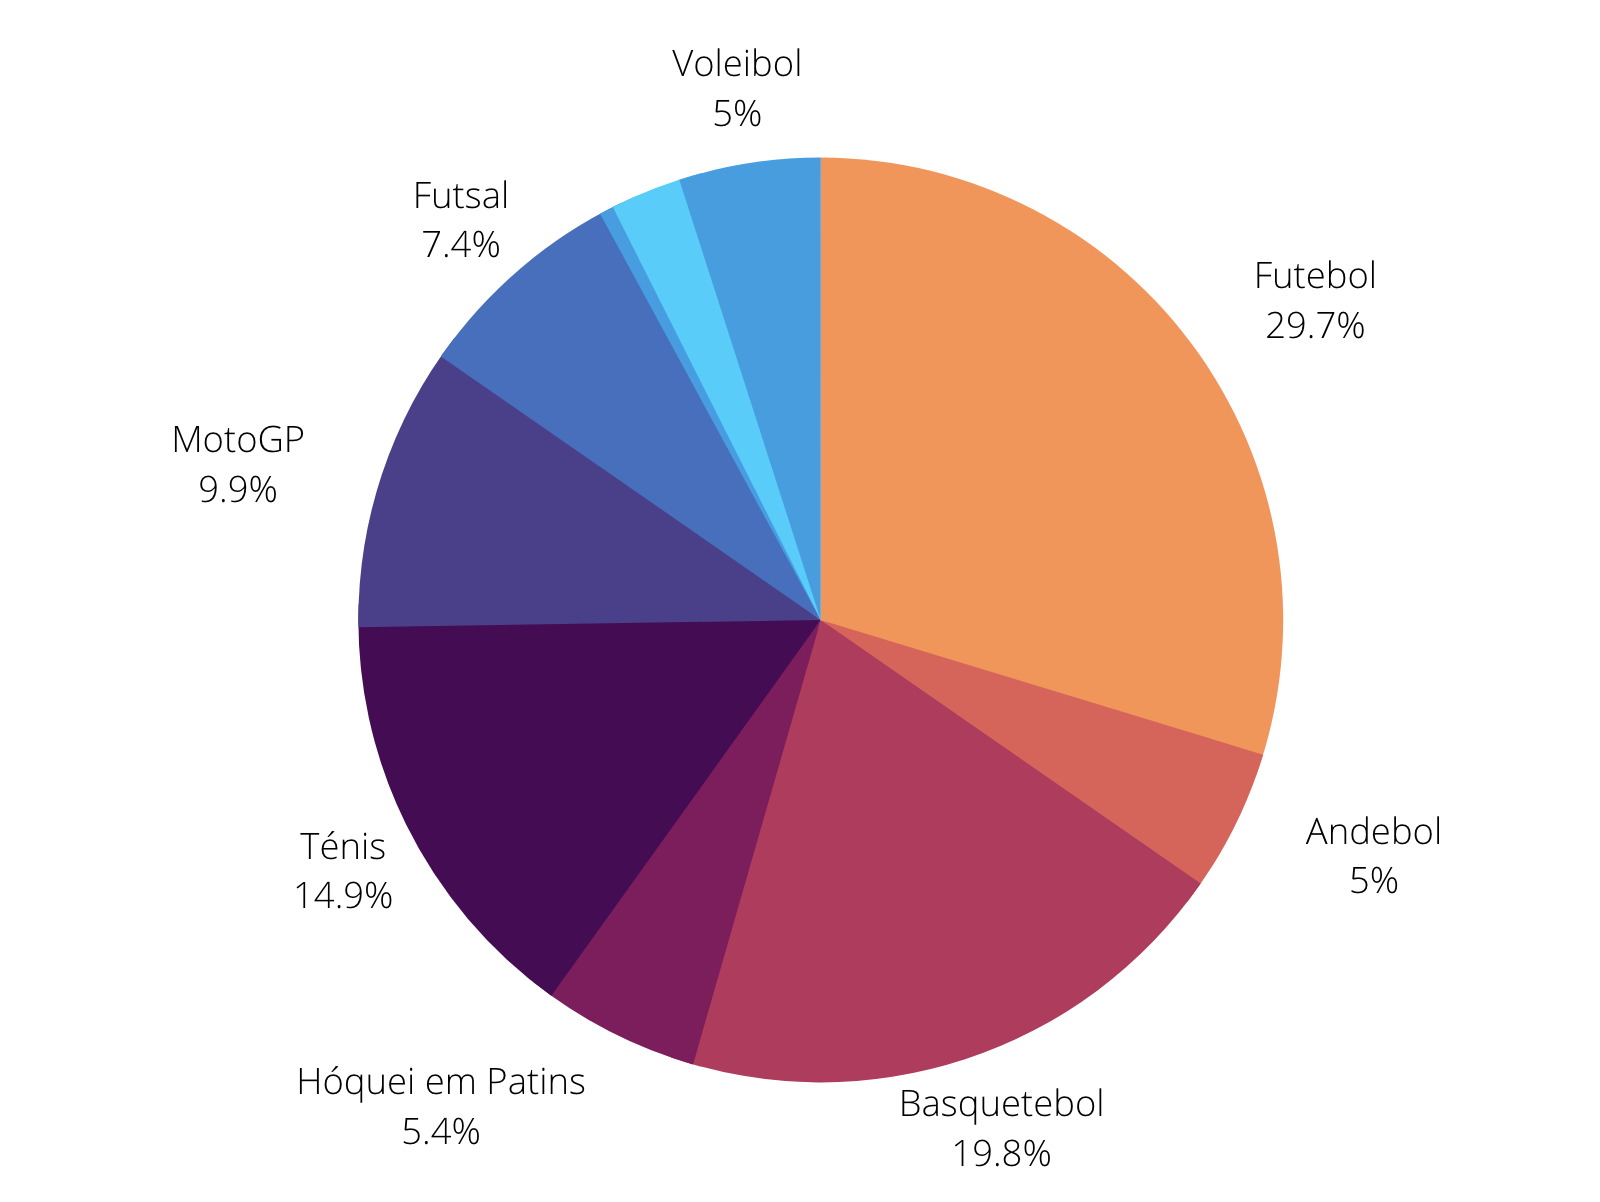
\includegraphics[width=.65\linewidth]{imagens/levantamentoRequisitos/Grafico1.png}
            \caption{Gráfico 1 }
        \end{figure}
    \vspace{20mm}
    \item \textbf{Gostavam de apostar em...}
        \begin{figure}[!htb]
            \centering
            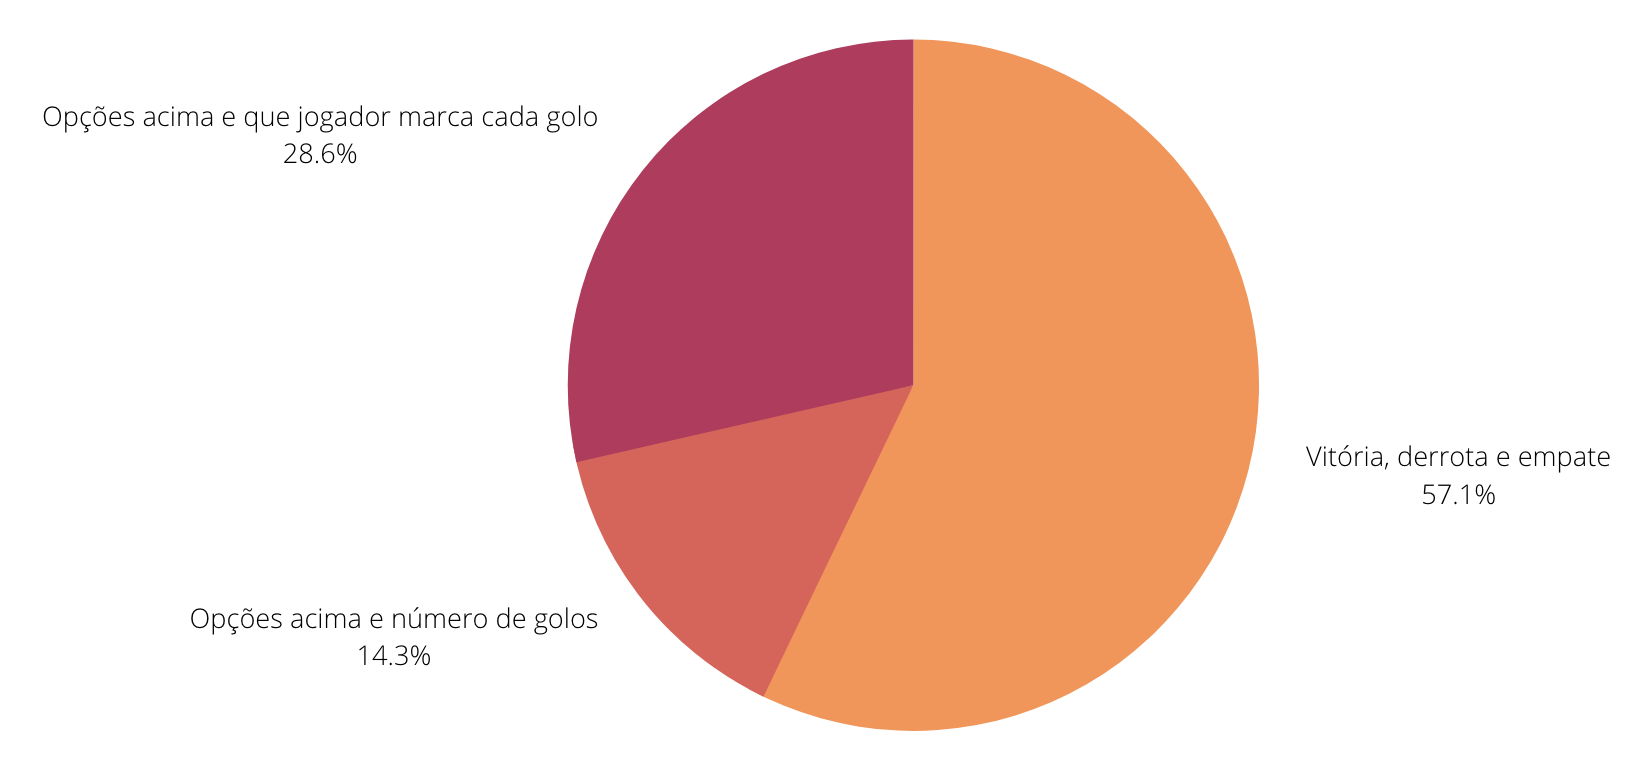
\includegraphics[width=.90\linewidth]{imagens/levantamentoRequisitos/Grafico2.png}
            \caption{Gráfico 2 }
        \end{figure}
        \newpage
    \item \textbf{Gostavam de ter hipótese de fazer mais de uma aposta simultaneamente?}
        \begin{figure}[!htb]
            \centering
            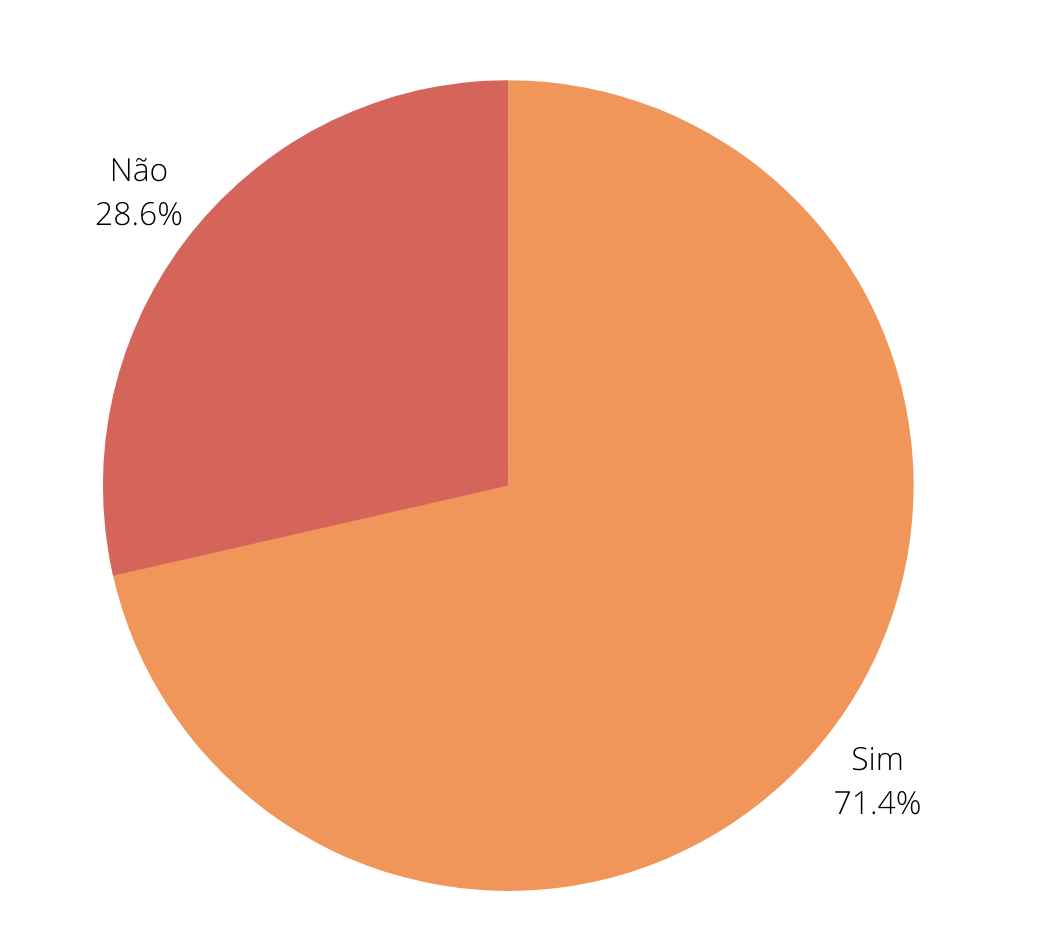
\includegraphics[width=.50\linewidth]{imagens/levantamentoRequisitos/Grafico3.png}
            \caption{Gráfico 3 }
        \end{figure}
\end{enumerate}

\subsection{Entrevista ao diretor da casa de apostas}
A presente entrevista foi elaborada pelos elementos do grupo, de modo a obter informações acerca das necessidades dos nossos clientes, as casas de apostas.
\subsubsection{Transcrição da Entrevista}
Entrevista conduzida ao diretor da casa de apostas \textit{DiBet}.
\begin{itemize}
    \item[] \texttt{ENTREVISTADOR:} Que tipos de desportos é que gostaria de ver no sistema?
    \item[] \texttt{ENTREVISTADO:} Como é de conhecimento geral, o futebol é o desporto mais praticado e adorado do mundo, portanto penso que será indispensável a sua inclusão. Para além deste, considero o basquetebol uma aposta muito interessante e segura a ser considerada. 
    
    \item[] \texttt{ENTREVISTADOR:} Considera a criação de um serviço web ou mobile futuramente uma abordagem interessante?
    \item[] \texttt{ENTREVISTADO:} Sem dúvida, penso que a criação de um serviço web é indispensável. Desta forma, os apostadores podem aceder ao serviço de apostas em qualquer equipamento.
    
    \item[] \texttt{ENTREVISTADOR:} Gostaria que a equipa de programadores estivesse disponível para dar suporte à aplicação criada futuramente?
    \item[] \texttt{ENTREVISTADO:} Sim, conto com uma equipa que esteja disponível para dar assistência ao sistema e para futuramente expandi-lo. 
    
    \item[] \texttt{ENTREVISTADOR:} Considera importante o sistema expandir as apostas a outros desportos consoante a demanda?
    \item[] \texttt{ENTREVISTADO:} Sim, dependendo da afluência dos meus clientes ao sistema pode ser interessante ter um sistema mais abrangente.
\end{itemize}

\subsubsection{Resumo} A entrevista conduzida ao diretor da casa de apostas foi muito esclarecedora, deu-nos uma ideia mais concreta do que é indispensável incluir no sistema a ser desenvolvido assim como o que pode vir a ser escalável.

\section{Personas}

\subsection{Persona Carlos Moreira} 

\textbf{Nome: }Carlos Moreira 

\textbf{Idade: }30 anos

\textbf{Estado Civil: }Solteiro

\textbf{Habilitações Académicas: }Mestrado em Engenharia Biomédica

\textbf{Profissão: }Engenheiro Biomédico

\textbf{Hobbies: }Fazer apostas desportivas online

\textbf{Residência: }Reside sozinho em Esposende\vspace{5mm}

\textbf{Estilo de vida: } O Carlos é um homem dedicado à sua profissão, trabalha arduamente todo dia. Quando chega a casa, sozinho e com poucos amigos, dedica-se a estudar jogos de basquetebol para fazer as melhores apostas. Sempre adorou o desporto porém o trabalho levou a melhor e já não pratica tanto como gostaria. 


\subsection{Persona João Silva} 

\textbf{Nome: } João Silva

\textbf{Idade: }26 anos

\textbf{Estado Civil: }Solteiro

\textbf{Habilitações Académicas: } 12º Ano

\textbf{Profissão: } Assistente de Oficina Automóvel

\textbf{Hobbies: } Ver MotoGP, Futebol, jogar futebol.

\textbf{Residência: }Reside com os pais em Lisboa\vspace{5mm}

\textbf{Estilo de vida: } O João é amante de um estilo de vida boémio, apreciador da vida noturna. Quando não se encontra na oficina, dedica-se a ver videos no youtube sobre desportos motorizados e futebol, tentando sempre antecipar o resultado dos eventos no fim de semana. Sempre teve o sonho de ser piloto de motociclos, ainda que desde cedo, percebeu que muito dificilmente teria as oportunidades necessárias em Portugal, dedicando-se assim ao ofício de reparação e preparação de carros e motas.

\subsection{Persona Joana Melo} 

\textbf{Nome: } Joana Melo

\textbf{Idade: }36 anos

\textbf{Estado Civil: } Casada

\textbf{Habilitações Académicas: } Licenciada em Ciências da Comunicação

\textbf{Profissão: } Gerente de Loja de Fotografia, blogger em part-time.

\textbf{Hobbies: } Fazer yoga, ver futebol, Fotógrafa amadora, blogger.

\textbf{Residência: }Reside com o marido no Algarve\vspace{5mm}

\textbf{Estilo de vida: } Fanática por futebol e fotografia desde jovem, a Joana acompanha regularmente eventos de futebol nacionais e europeus, sendo uma paixão que partilha com o seu marido. 

\section{Introspeção}
Nesta secção foi feito o levantamento de requisitos através de diferentes estratégias definidas pelos elementos da equipa. Este levantamento foi realizado, agregado e por fim, foi selecionada a informação mais relevante para o projeto em questão.
\par
As entrevistas feitas foram revistas e validadas de forma a verificar se reúnem as características necessárias das partes interessadas. Destes passos resulta um conjunto de requisitos importantes a implementar na nossa aplicação.